\subsection*{Modello 1: v8m12 e v8m12bis}

% Introduzione su strategia del training -> qual è l'obiettivo dell'esperimento?
I primi esperimenti sono serviti per raccogliere informazioni utili per avere un fase di 
addestramento che fosse il più efficacie possibile. Innanzitutto si è cercato di capire quanto
tempo avrebbe ogni iterazione, ogni epoca e in genere l'addestramento richiesto e capire 
in particolare quante risorse computazionali erano richieste e quante epoche consentire
al modello durante la fase di training.

Questi test, così come molti dei seguenti esperimenti, sono stati eseguiti su un notebook
jupiter eseguito su server colab, sfruttando l'accelerazione GPU, in genere una scheda T4, 
fornita giornalmente per un massimo di 3 ore da parte di Google.

% Dettagli configurazione, tipologia modello e iperparametri

Una delle prime prove svolte riguarda due esecuzioni di training denominate durante il lavoro
\verb+v8m12+ e \verb+v8m12bis+. La prima è stata un'esecuzione di sole 30 epoche per vedere quanto 
velocemente le funzioni di loss scendessero di valore e stimare quante epoche concedere successivamente.
Il modello utilizzato è quello medio preaddestrato con il dataset COCO, come disponibile dalla libreria 
di ultralytics (YOLOv8m.pt).
La seconda esecuzione ha visto sempre un numero di epoche pari a 30 ma utilizzando come modello di
partenza il miglior modello dell'addestramento precedente in quanto dai risultati come è possibile vedere 
nella figura \ref{fig:v1-1} c'era ancora margine di miglioramento.

\begin{figure}[h]
    \centering
    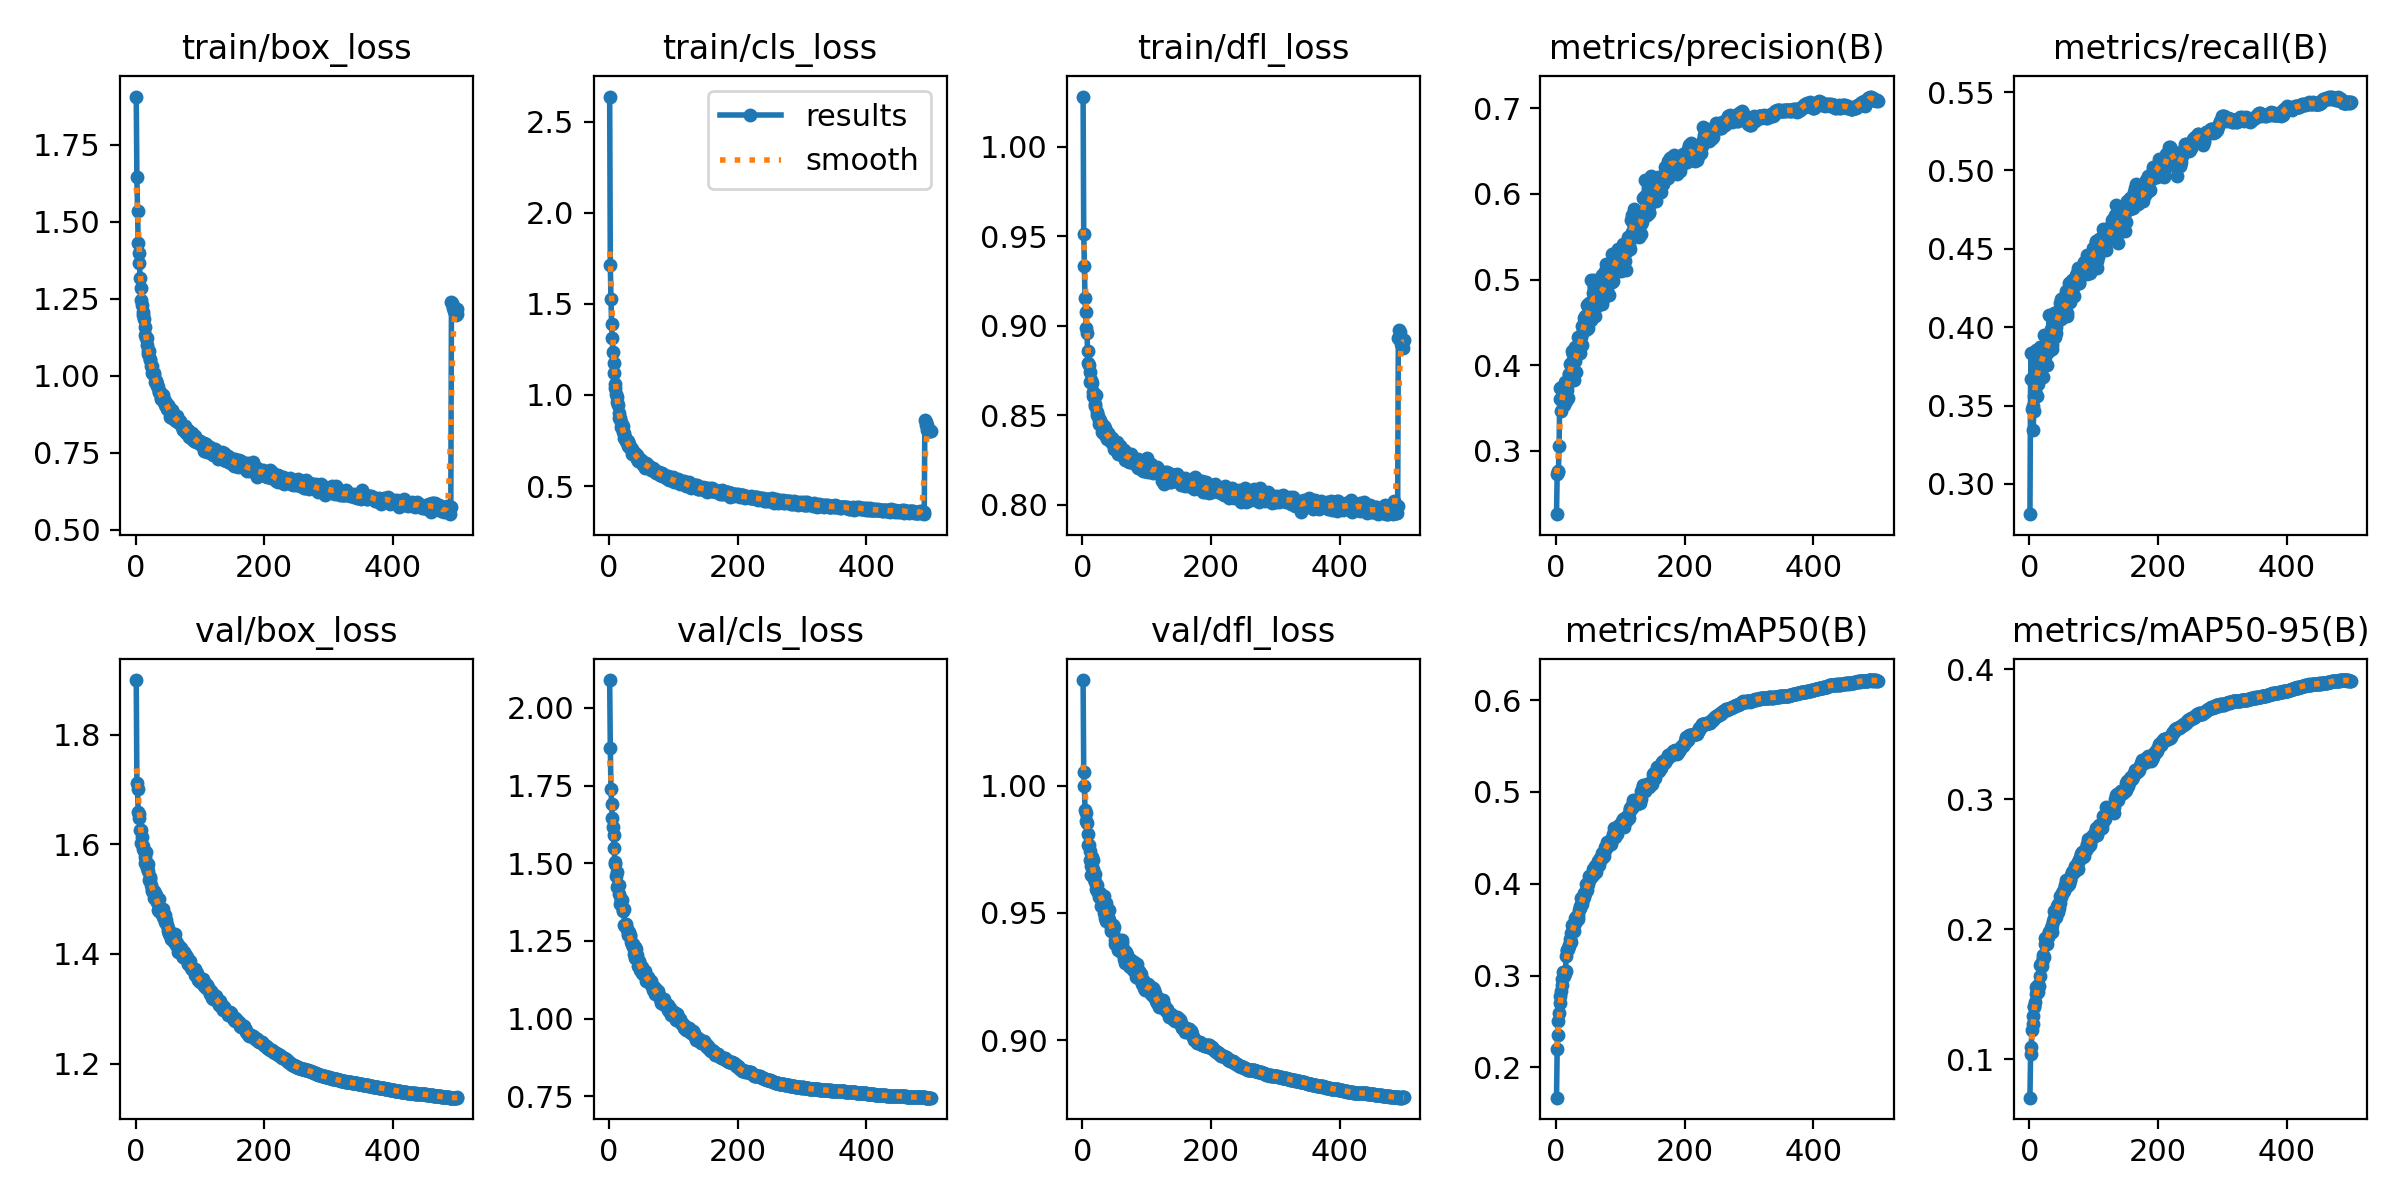
\includegraphics[width=0.8\textwidth]{v_1/results.png}
    \caption{Andamento funzioni di loss e metriche durante l'esecuzione di v8m12}
    \label{fig:v1-1}
    \end{figure}

Molti degli iperparametri, se non tutti, sono stati tenuti quelli di default della libreria di ultralytics.
L'unico iperparametro impostato per curiosità è \verb|freeze|: in breve abbiamo tenuto 7 layer del modello 
di yolo congelati in modo da ridurre il tempo necessario per l'addestramento. Per la bontà dell'esperimento
si è dimostrato di poca utilità e gli addestramenti successivi tale iperparametro è stato ignorato, 
ovvero la modifica dei pesi avveniva su tutto il modello.

% Risultati training
    % - andamento training
    % - grafici recall e precision e performance e F1
    % - matrici di confusione
    % - tabella performance test set

% Commento risultati

In ogni caso a prescindere dai risultati ottenuti, che per la natura dell'esperimento non sono
fondamentali, si è visto come il numero di epoche necessario per 
l'addestramento dovrebbe essere molto più alto per poter raggiungere quanto meno un'efficacia del modello
accettabile, così come è stato fatto poi per gli esperimenti successivi.